\documentclass[conference]{IEEEtran}
\IEEEoverridecommandlockouts
% The preceding line is only needed to identify funding in the first footnote. If that is unneeded, please comment it out.
\usepackage{cite}
\usepackage{amsmath,amssymb,amsfonts}
\usepackage{algorithmic}
\usepackage{graphicx}
\usepackage{textcomp}
\usepackage{xcolor}
\usepackage{placeins}
\usepackage[hidelinks]{hyperref}
\usepackage{float}
\usepackage{subcaption}
\def\BibTeX{{\rm B\kern-.05em{\sc i\kern-.025em b}\kern-.08em
    T\kern-.1667em\lower.7ex\hbox{E}\kern-.125emX}}
\begin{document}

\title{Redes Neurais Convolucionais}

\author{\IEEEauthorblockN{Arthur Abrahão Santos Barbosa}
\IEEEauthorblockA{\textit{Universidade Federal de Pernambuco} \\
\textit{Centro de Informática}\\
Pernambuco, Brasil \\
aasb2@cin.ufpe.br}
\and
\IEEEauthorblockN{Arthur Henrique}
\IEEEauthorblockA{\textit{Universidade Federal de Pernambuco} \\
\textit{Centro de Informática}\\
Pernambuco, Brasil \\
ahac@cin.ufpe.br}
\and
\IEEEauthorblockN{Filipe Samuel da Silva}
\IEEEauthorblockA{\textit{Universidade Federal de Pernambuco} \\
\textit{Centro de Informática}\\
Pernambuco, Brasil \\
fss8@cin.ufpe.br}
\and
\IEEEauthorblockN{Vinicius Bastos Moreira Principe}
\IEEEauthorblockA{\textit{Universidade Federal de Pernambuco} \\
\textit{Centro de Informática}\\
Pernambuco, Brasil \\
vbmp@cin.ufpe.br}
}

\maketitle



% \begin{abstract}
%     This document is a model and instructions for \LaTeX.
%     This and the IEEEtran.cls file define the components of your paper [title, text, heads, etc.]. *CRITICAL: Do Not Use Symbols, Special Characters, Footnotes, 
%     or Math in Paper Title or Abstract.
%     \end{abstract}
    
% \begin{IEEEkeywords}
% component, formatting, style, styling, insert
% \end{IEEEkeywords}




\section{Introdução}
Acidentes de trânsito são inesperados e causam diversas perdas. Existem diversas variáveis que contribuem com a gravidade
de um acidente.


\section{Base de Dados}

A base de dados vieram da junção das bases de acidentes de trânsito\cite{incidents}
ocorridos no Condado de Montgomery - Maryland, EUA e das informações dos motoristas envolvidos neste acidente\cite{drivers}.
Estas informações foram registradas pelo Sistema automatizado de Relatórios de acidentes da Policial estadual de Maryland.  

\subsection{Escopo e Seleção dos Dados}
Como definido pela base de dados, o escopo é dado apenas pelos acidentes de trânsito que ocorreram no Condado de Montgomery. 
\subsection{Definição do Objetivo}


\subsection{Pré Processamento dos Dados}
% Originalmente planejava-se definir a gravidade do acidente, caso tenha ou não casualidades.
% O processo foi definido inicia
Após a junção dos datasets, foram obtidas 77 colunas de atributos, porém existia colunas com muitos valores nulos que foram 
substituidas para "False" ou removidas e também muita  informação a posterióri que necessitavam ser removidas.
Considerando as restrições de captação de dados do veículo, foram incluidos apenas os atributos mais significativos e pertinentes para a análise, 
enquanto outras colunas foram agrupadas, para melhor organizar os dados restando menos das metades features para serem analisadas. 

\subsection{Definição do Alvo}
O alvo da classificação binária foi definido em relação ao dano do veículo, e o Objetivo é descobrir se houve ou não da
no significativo ao veículo durante o acidente.
\section{Extração de Dados, Resultados e Discussão}
Para extrair o conhecimento inserido na base de dados, 
foram utilizados três métodos: regressão logistica, arvore de decisão, e indução de regras
\subsection{Regressão Logistica}
Após treinar o modelo de regressão logistica, foram analisadas as features com maior coeficiente beta, e que possuíssem maior 
significância de acordo com o p-valor, onde os coeficientes de maior módulo tem mais relevância ao definir a classe alvo.
As features com maior valor positivo tem maior contribuição para definir que houve
dano significativo ao veículo, enquanto as de valores mais negativos possuem uma importância maior para definir se não houve dano significativo.

Se o carro está se movendo ou é particular há uma maior chance de possuir dano significativo após o acidente, enqunto se tiver algum não motorista
participando do acidente (pedestre ou ciclista), se o carro estiver acelerando ou se a colisão for na mesma direção, a probabilidade de 
não haver dano significativo é bem menor.

\begin{table}[!ht]
    \centering
    \begin{tabular}{|l|l|l|l|l|l|l|l|l|l|}
    \hline
        Feature~ & Beta~ & ~p-valor  \\ \hline
        is\_moving~ &  1.259~ & ~0  \\ \hline
        is\_particular~ & 1.255~ & ~0  \\ \hline
        RelatedNon-Motorist ~ & -2.652~ & ~0  \\ \hline
        is\_accelerating ~ & -1.212 ~ & ~0  \\ \hline
        CollisionType=SameDir ~ & -1.175 ~ & ~0  \\ \hline
    \end{tabular}
\end{table}



\begin{figure}[H]
    \centerline{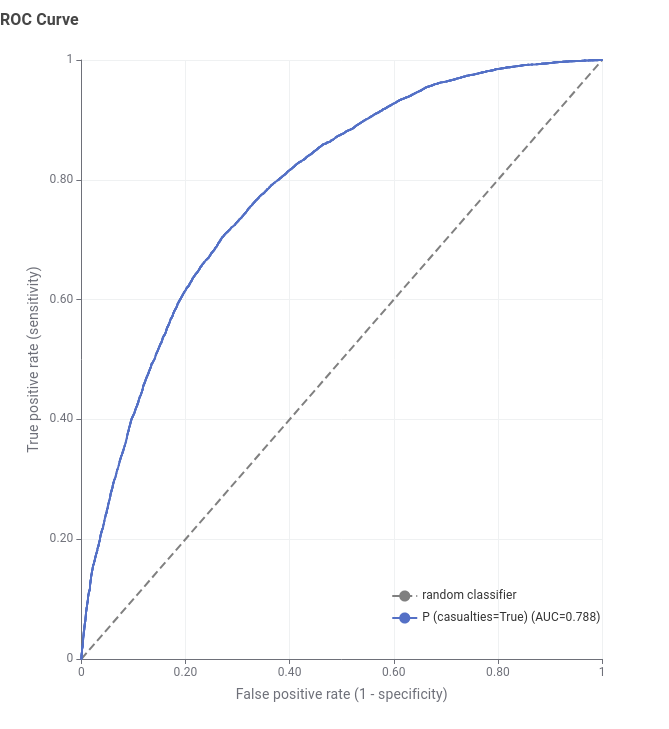
\includegraphics[width=0.4\textwidth]{Images/roc-curve-regressor.png}}
    \caption{\label{fig:decision-tree} Curva ROC Para o Regressor Logistico}
\end{figure}

\subsection{Árvore de Decisão}

A árvore de decisão é um dos modos mais simples de visualisar o conhecimento presente em uma 
base de dados de modo compreenssivel. As variáveis mais importantes para definir a classe alvo foram...
\begin{figure}[H]
\centerline{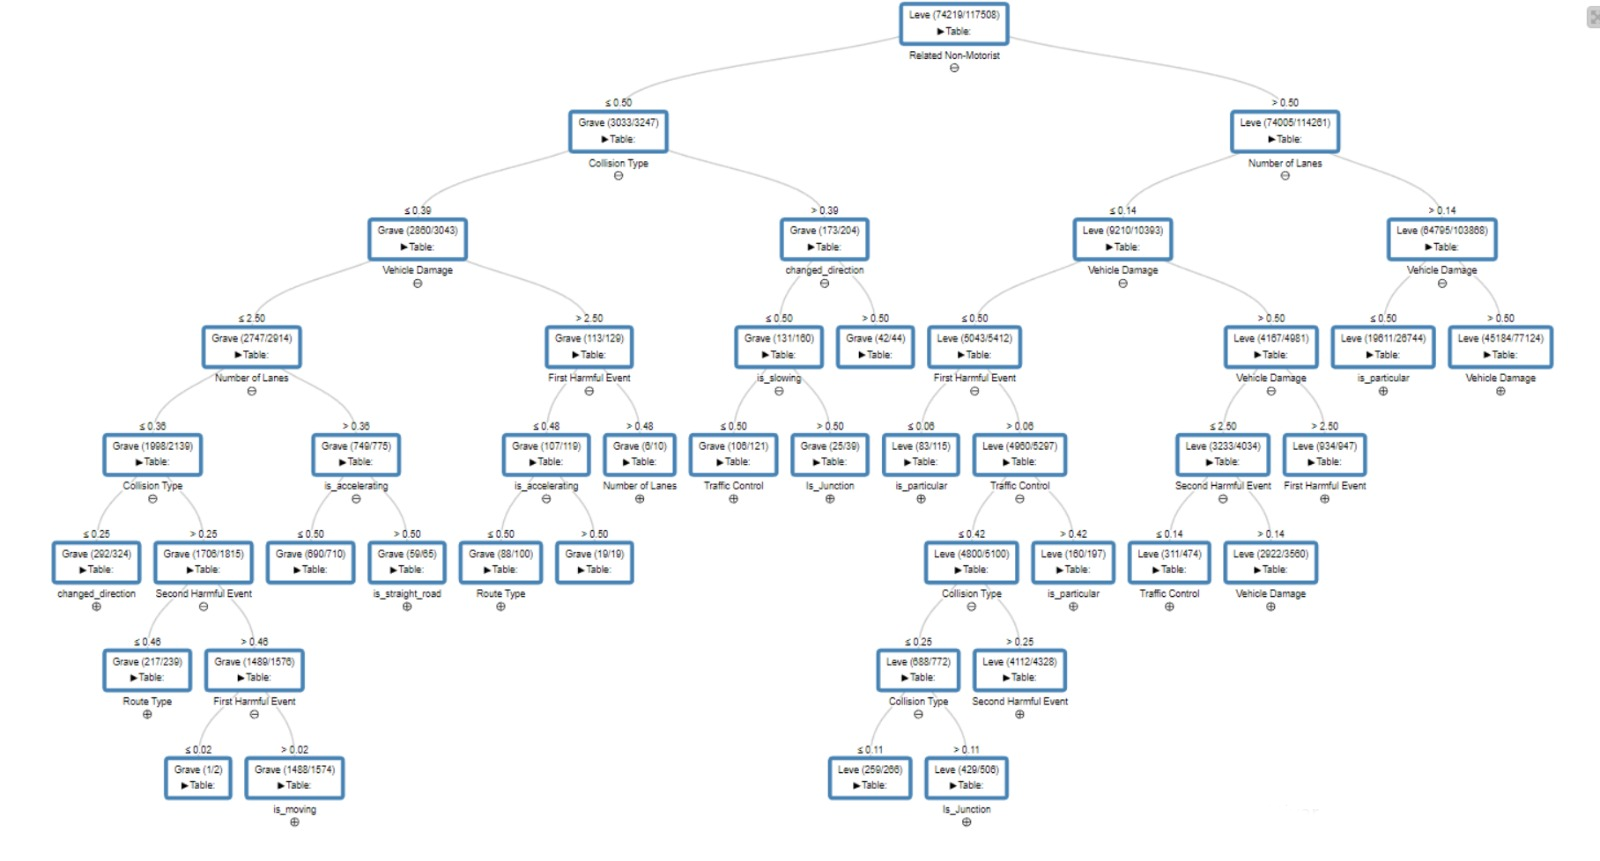
\includegraphics[width=0.4\textwidth]{Images/decision-tree.png}}
\caption{\label{fig:decision-tree} Árvore de decisão gerada usando o Knime}
\end{figure}

\begin{figure}[H]
    \centerline{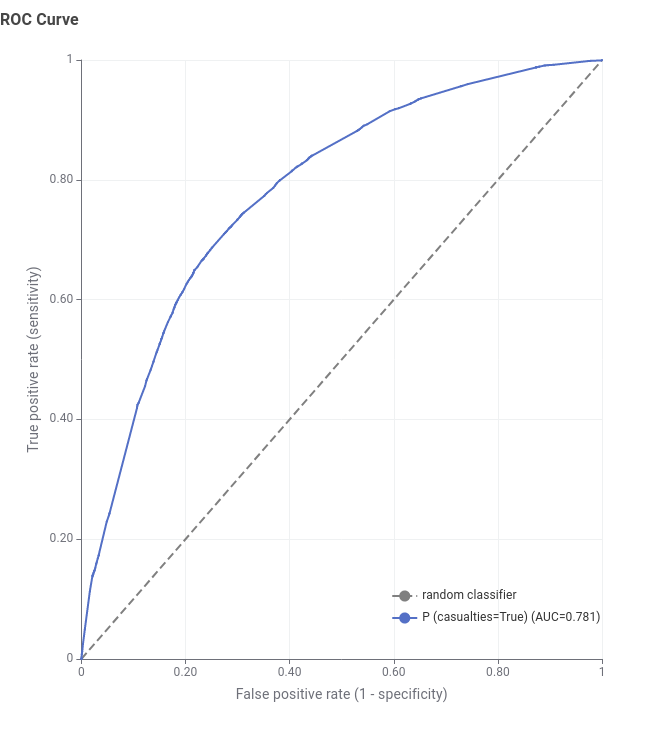
\includegraphics[width=0.4\textwidth]{Images/roc-curve-decision-tree.png}}
    \caption{\label{fig:decision-tree} Curva ROC Para a Árvore de Decisão}
\end{figure}


\subsection{Indução de Regras de Classificação}
% \subsection{Propensity score performance score}

\begin{table}[!ht]
    \centering
    \begin{tabular}{|l|l|l|l|l|l|l|l|l|l|}
    \hline
        Feature~ & Cobertura~ & ~Confiança & ~ Lift \\ \hline
        is\_moving~ &  1.259~ & ~0 & ~  \\ \hline
    \end{tabular}
    \caption{label{tab:tab2} HEre}
\end{table}
\section{Conclusão}



% \begin{figure}[H]
% \centerline{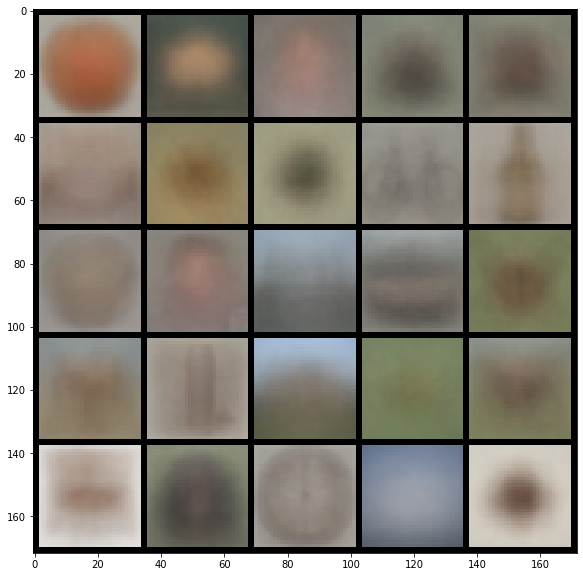
\includegraphics[width=0.4\textwidth]{Images/img_mean1.png}}
% \caption{\label{fig:img_mean1}Da esquerda para a direita, de cima para a baixo: apple, aquarium\_fish, baby, bear, beaver, bed, bee, beetle, bicycle, bottle, bowl, boy, bridge, bus, butterfly, camel, can, castle, caterpillar, cattle, chair, chimpanzee, clock, cloud, cockroach}
% \end{figure}

% \begin{figure}[H]
% \centerline{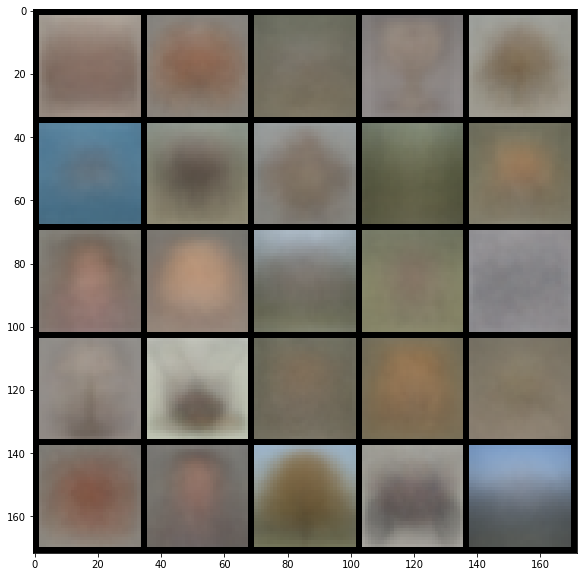
\includegraphics[width=0.4\textwidth]{Images/img_mean2.png}}
% \caption{\label{fig:img_mean2}Da esquerda para a direita, de cima para a baixo: couch, crab, crocodile, cup, dinosaur, dolphin, elephant, flatfish, forest, fox, girl, hamster, house, kangaroo, keyboard, lamp, lawn\_mower, leopard, lion, lizard, lobster, man, maple\_tree, motorcycle, mountain}
% \end{figure}

% \begin{figure}[H]
% \centerline{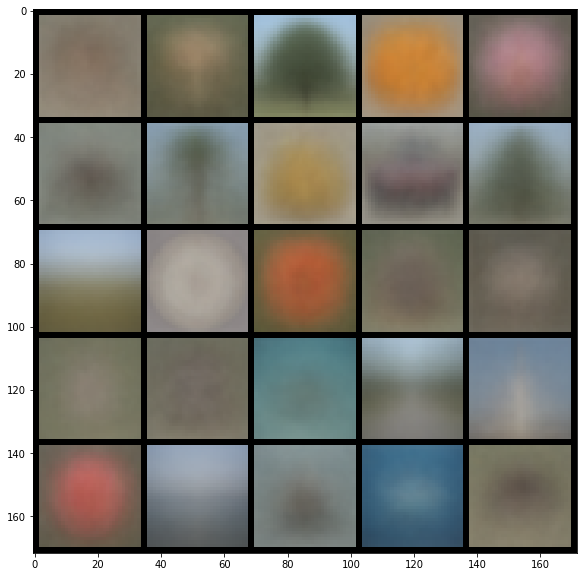
\includegraphics[width=0.4\textwidth]{Images/img_mean3.png}}
% \caption{\label{fig:img_mean3}Da esquerda para a direita, de cima para a baixo: mouse, mushroom, oak\_tree, orange, orchid, otter, palm\_tree, pear, pickup\_truck, pine\_tree, plain, plate, poppy, porcupine, possum, rabbit, raccoon, ray, road, rocket, rose, sea, seal, shark, shrew}
% \end{figure}

% \begin{figure}[H]
% \centerline{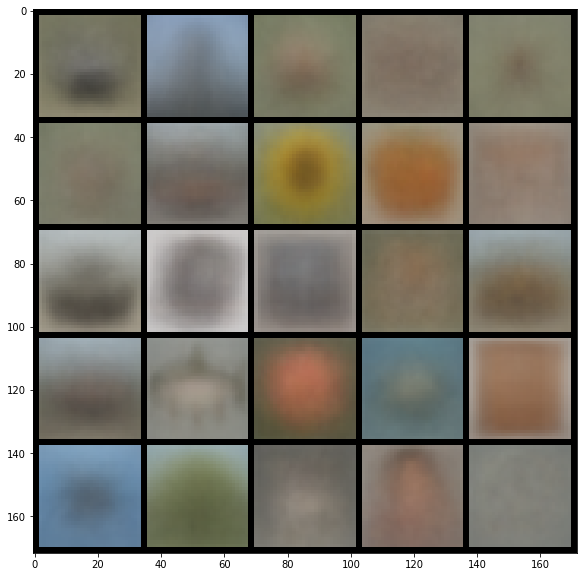
\includegraphics[width=0.4\textwidth]{Images/img_mean4.png}}
% \caption{\label{fig:img_mean4}Da esquerda para a direita, de cima para a baixo: skunk, skyscraper, snail, snake, spider, squirrel, streetcar, sunflower, sweet\_pepper, table, tank, telephone, television, tiger, tractor, train, trout, tulip, turtle, wardrobe, whale, willow\_tree, wolf, woman, worm}
% \end{figure}

% \begin{itemize}
% \item Média da Imagens Normalizadas
% \end{itemize}

% \begin{figure}[H]
% \centerline{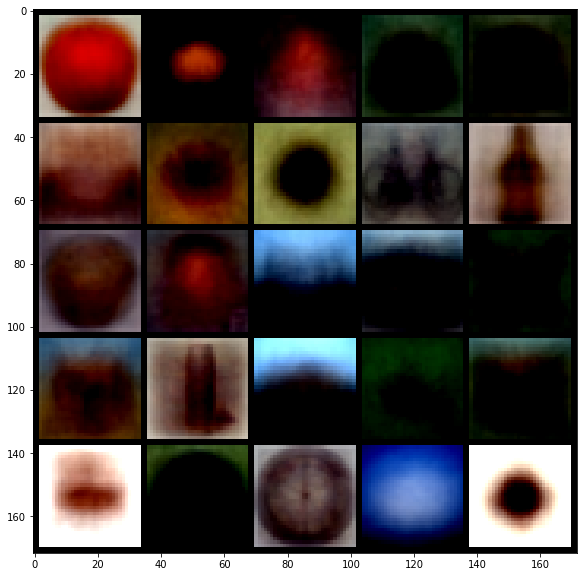
\includegraphics[width=0.4\textwidth]{Images/img_mean_norm1.png}}
% \caption{\label{fig:img_mean_norm1}Da esquerda para a direita, de cima para a baixo: apple, aquarium\_fish, baby, bear, beaver, bed, bee, beetle, bicycle, bottle, bowl, boy, bridge, bus, butterfly, camel, can, castle, caterpillar, cattle, chair, chimpanzee, clock, cloud, cockroach}
% \end{figure}

% \begin{figure}[H]
% \centerline{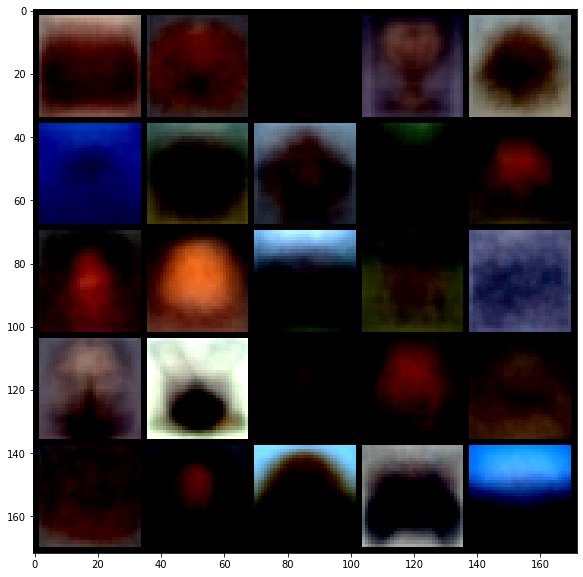
\includegraphics[width=0.4\textwidth]{Images/img_mean_norm2.png}}
% \caption{\label{fig:img_mean_norm2}Da esquerda para a direita, de cima para a baixo: couch, crab, crocodile, cup, dinosaur, dolphin, elephant, flatfish, forest, fox, girl, hamster, house, kangaroo, keyboard, lamp, lawn\_mower, leopard, lion, lizard, lobster, man, maple\_tree, motorcycle, mountain}
% \end{figure}

% \begin{figure}[H]
% \centerline{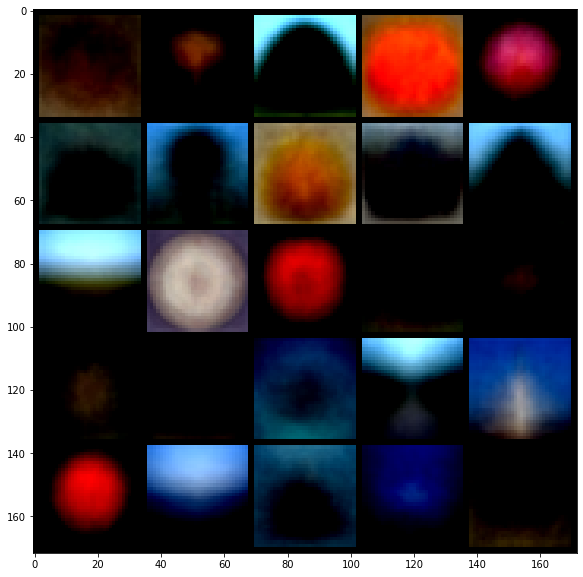
\includegraphics[width=0.4\textwidth]{Images/img_mean_norm3.png}}
% \caption{\label{fig:img_mean_norm3}Da esquerda para a direita, de cima para a baixo: mouse, mushroom, oak\_tree, orange, orchid, otter, palm\_tree, pear, pickup\_truck, pine\_tree, plain, plate, poppy, porcupine, possum, rabbit, raccoon, ray, road, rocket, rose, sea, seal, shark, shrew}
% \end{figure}

% \begin{figure}[H]
% \centerline{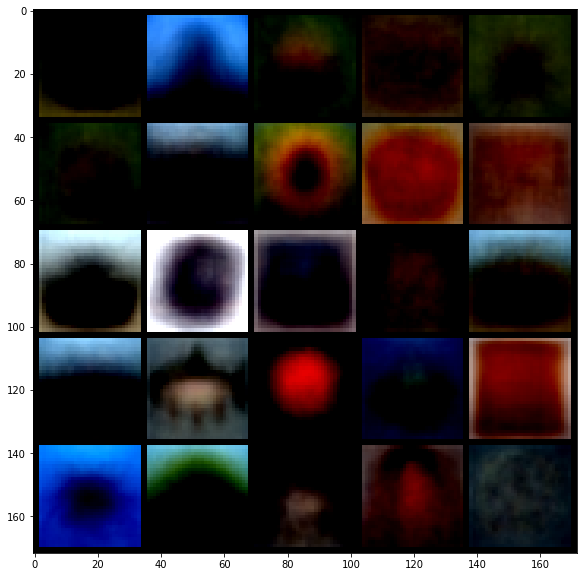
\includegraphics[width=0.4\textwidth]{Images/img_mean_norm4.png}}
% \caption{\label{fig:img_mean_norm4}Da esquerda para a direita, de cima para a baixo: skunk, skyscraper, snail, snake, spider, squirrel, streetcar, sunflower, sweet\_pepper, table, tank, telephone, television, tiger, tractor, train, trout, tulip, turtle, wardrobe, whale, willow\_tree, wolf, woman, worm}
% \end{figure}
    
%\subsection{Sobre o Projeto}
%Para montar o classificador foi necessário passar  pelas seguintes etapas:



% \section{Sobre as Métricas Utilizadas}

% \subsection{Precision}

% Precision é a razão
%     \begin{equation}
%         \frac{A_c}{A_c + A_e}
%     \end{equation}

%     onde:

%     \begin{itemize}
%     \item $A_c$ é o número de amostras corretamente classificadas de uma determinada classe.
%     \item $A_e$ é o número de amostras  erroneamente classificadas como sendo desta determinada classe.
%     \end{itemize}

%     Precision é intuitivamente a habilidade do classificador não marcar como pertencente a uma classe uma amostra que não pertence a esta. O melhor valor de Precision é 1 e o pior é zero.
%     \cite{b7}
% \subsection{Accuracy} 

% Accuracy é a fração de amostras preditas corretamente, e é dada pela seguinte fórmula:

% \begin{equation}
%     \frac{\sum\limits_{1}^{n}A_c}{\sum\limits_{1}^{n}A_t}
% \end{equation}







\bibliography{mybib}
\nocite{*}
\bibliographystyle{IEEEtran}
\end{document}
